
\documentclass[journal=inoraj,manuscript=article]{achemso}
\usepackage[version=3]{mhchem} % Formula subscripts using \ce{}
\usepackage[T1]{fontenc}       % Use modern font encodings
\usepackage{color}
\usepackage{subcaption}
\usepackage{epstopdf}
\usepackage{epsfig}
\usepackage{graphicx}
%\usepackage[format=hang,singlelinecheck=0,font={sf,small},labelfont=it]{subfig}
\usepackage{caption}
\usepackage{bm}
\usepackage{mciteplus}
\setkeys{acs}{articletitle = true}

\title{EDA analysis SHE}
\author{Leonardo Belpassi}

\author{Loriano Storchi}
\date{November 2022}

\begin{document}

\maketitle

\section{Introduction}

\section{Theoretical background and computational details}

Here some details and a test using ADF vs light atom

\section{A case study the AuX+ (X=Hg, Pb, Rn, Cn, Fl, Og) systems  }

The large component of the basis set was generated by decontracting triple-z quality Dyall’s basis sets~\cite{missedref} 
augmented with the related polarization and correlating functions. Final basis set schemes are as follows:
 Hg and Au (30s 24p 15d 11f 5g 1h), Cn (32s 29p 20d 14f 7g 2h), Pb and Rn (31s 27p 18d 12f 4g 1h), Fl and Og (31s 30p 21d 14f 6g 2h).
 The corresponding small component basis was generated using the restricted kinetic balance relation~\cite{missedref}.

\begin{table}[!h]
\begin{tabular}{lr}
\hline
  System    & Coulomb energy \\
            & absolute error (a.u.) \\
\hline
  AuHg$^+$ & $ 7.9544 10^{-6}$ \\ \hline
  AuCn$^+$ &$ 7.9544 10^{-6}$ $ 3.0342 10^{-6}$ \\ \hline
  AuPb$^+$ &$ 7.9544 10^{-6}$ $ 5.5167 10^{-6}$ \\ \hline
  AuFl$^+$ &$ 7.9544 10^{-6}$ $ 9.0849 10^{-6}$ \\ \hline
  AuRn$^+$ &$ 7.9544 10^{-6}$ $ 1.8594 10^{-5}$ \\ \hline
  AuOg$^+$ &$ 7.9544 10^{-6}$ $ 6.0255 10^{-6}$ \\ \hline
\end{tabular}
  \caption{Absolute error of the coulomb energy calculated using the density fitting procedure
   with respect the exact coulomb energy}
  \label{energydiff}
\end{table}



 For gold, a previously optimized auxiliary basis set for density density fitting denoted as B20 was used~\cite{missedref}. For all other 
 elements, we devised a simple scheme in order to generate the auxiliary fitting basis sets. For each element we explicitly consider 
 the s-type exponents taken from double-z Dyall’s basis sets, augment with the related diffuse functions. Each exponent is doubled in magnitude. 
 As far as the angular part is concerned we adopted the following criterion: we associated l = 0 to the initial four exponents in the  list. Then all 
 exponents of order $\le$ 6.0 are related to l = 4. For all the remaining exponents in the list we set up l = 2.
 It is worth recalling that the sets are formed so that to an auxiliary function of a given angular momentum all the functions of smaller angular momentum 
 are associated. We
 assess the quality of fitting basis set evaluating the accuracy i
 (absolute error) of the coulomb energy calculated using the density fitting procedure 
 with respect the exact coulomb energy. (see Table \ref{energydiff})
The BLYP functional
made of Beck 1998 (B88) exchange \cite{missedref} plus the Lee-Yang-Parr (LYP) correlation \cite{missedref} was used. An energy convergence criterion of $10^-11$
Hartree 
on the total energy was adopted. 

All were obtained as results of numerical geometry optimization carried out with BERTHA

\begin{table}[!h]
\begin{tabular}{lrrrrrr}
\hline
                       & AuHg$^+$ & AuCn$^+$ & AuPb$^+$  & AuFl$^+$ & AuRn$^+$ & AuOg$^+$ \\ \hline
\hline
$\Delta E_{int}$       & -51.1341 & -35.1953 & -106.0481 & -65.6807 & -47.4012 & -69.6545 \\ \hline
$\Delta E_{ETS-Pauli}$ &  80.4823 &  79.0281 &  115.7724 &  72.1223 &  85.5963 &  81.6895 \\ \hline
$\Delta E_{exc}$       & -25.9427 & -24.3970 &  -31.8787 & -19.9776 & -24.0878 & -23.3315 \\ \hline
$\Delta E_{Pauli}$     &  54.5396 &  54.6311 &   83.8937 &  52.1447 &  61.5084 &  58.3580 \\ \hline
$\Delta E_{Elect}$     & -42.5393 & -39.3235 &  -65.0604 & -39.1422 & -45.6129 & -46.2992 \\ \hline
$\Delta E_{orb}$       & -63.1344 & -50.5030 & -124.8815 & -78.6832 & -63.2968 & -81.7133 \\ \hline
$\Delta E_1$           & -54.2088 & -38.3577 & -110.5783 & -68.6034 & -49.8713 & -71.7696 \\ \hline
$\Delta E_2$           &  -4.3425 &  -5.5161 &   -2.5708 &  -4.5726 &  -6.0586 &  -4.0202 \\ \hline
$\Delta E_3$           &  -1.0651 &  -2.4930 &   -6.2776 &  -1.4079 &  -4.0528 &  -3.5042 \\ \hline
$\Delta E_4$           &  -1.3728 &  -0.8403 &   -3.1012 &  -1.7332 &  -2.5051 &  -1.4569 \\ \hline
$\Delta E_5$           &  -0.8896 &  -1.6396 &   -0.9819 &  -0.4289 &  -0.1444 &  -0.3208 \\ \hline
$\Delta E_6$           &  -0.4682 &  -0.0176 &   -0.1823 &  -0.0551 &  -0.1193 &  -0.1734 \\ \hline
\end{tabular}
\caption{EDA analysis for AuX$^+$ systems}
\end{table}

\begin{table}[!h]
\begin{tabular}{lrrrrrr}
\hline
                 & AuHg$^+$  & AuCn$^+$  & AuPb$^+$  & AuFl$^+$  & AuRn$^+$  & AuOg$^+$ \\ \hline
\hline
$CT_{nocv1}$     &  0.477012 &  0.361730 &  0.963528 &  0.714536 &  0.490026 &  0.686910 \\ \hline
$CT_{nocv2}$     &  0.000208 & -0.052032 & -0.093912 & -0.027708 & -0.023532 & -0.024638 \\ \hline
$CT_{nocv3}$     & -0.006694 &  0.002634 & -0.055482 & -0.031918 &  0.003218 &  0.006910 \\ \hline
$CT_{nocv4}$     & -0.001326 & -0.006906 & -0.015444 & -0.008188 & -0.007912 & -0.014378 \\ \hline
$CT_{nocv5}$     &  0.002366 &  0.000786 &  0.006334 &  0.003400 & -0.012522 & -0.018664 \\ \hline
$CT_{nocv6}$     & -0.001138 & -0.004616 & -0.003668 & -0.002654 & -0.003216 & -0.002708 \\ \hline
$CT_{tot}$       &  0.435710 &  0.303804 &  0.799147 &  0.651476 &  0.450352 &  0.632027 \\ \hline
$CT_{tot ortho}$ &  0.461715 &  0.303098 &  0.800922 &  0.648890 &  0.442308 &  0.633309 \\ \hline
\end{tabular}
\caption{NOCV CT analysis for AuX$^+$ system}
\end{table}



\begin{figure}[!h]
\includegraphics[angle=-90,width=0.80\textwidth]{./AuHg+/cd.pdf}
\caption{CD curve for AuHg+ system}
\end{figure}

\begin{figure}[!h]
    \centering
    \centering
    \begin{subfigure}[t]{0.30\textwidth}
        \centering
        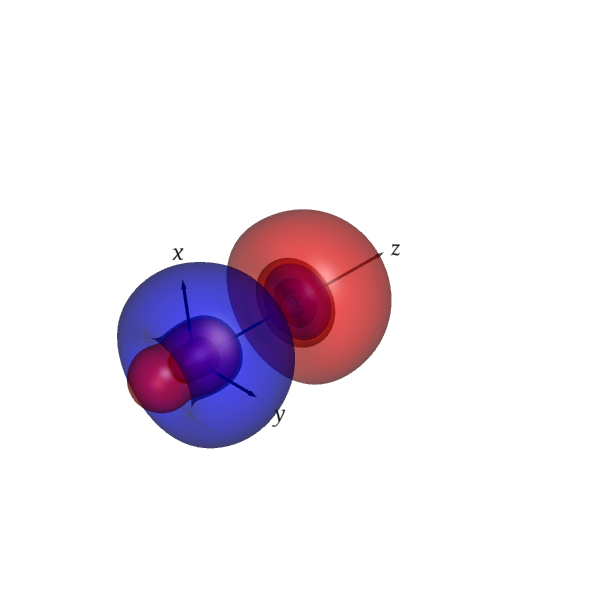
\includegraphics[width=0.8\linewidth]{./AuHg+/diff_tot.png} 
        \caption*{\ \ \ \ \ \ \ \ $\Delta \rho'$} 
    \end{subfigure}
    \hfill
 
    \vspace{0.0cm}
    \begin{subfigure}[t]{0.30\textwidth}
        \centering
        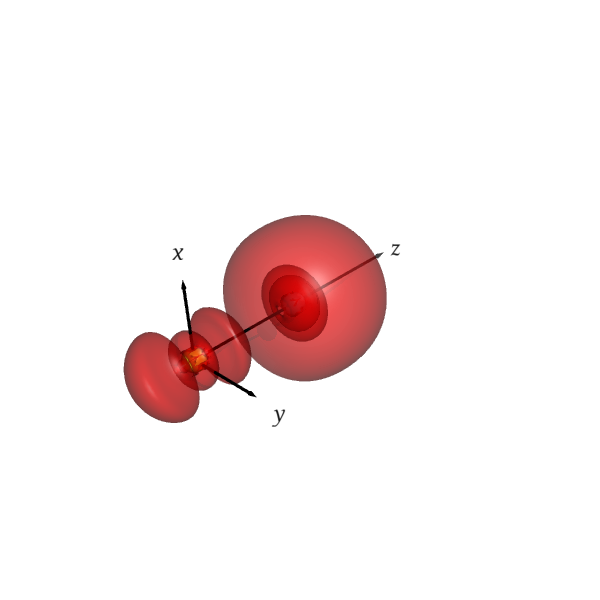
\includegraphics[width=\linewidth]{./AuHg+/nocv-1.png} 
        \caption*{\ \ \ \ \ \ \ \ $|\varphi_{-1}|^2$} 
    \end{subfigure}
    \hfill
    \begin{subfigure}[t]{0.30\textwidth}
        \centering
        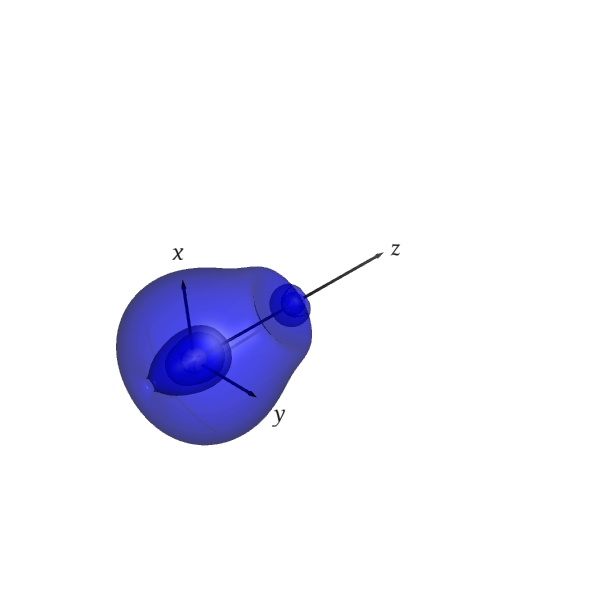
\includegraphics[width=\linewidth]{./AuHg+/nocv+1.png} 
        \caption*{\ \ \ \ \ \ \ \ $|\varphi_{+1}|^2$} 
    \end{subfigure}
    \hfill
    \begin{subfigure}[t]{0.30\textwidth}
        \centering
        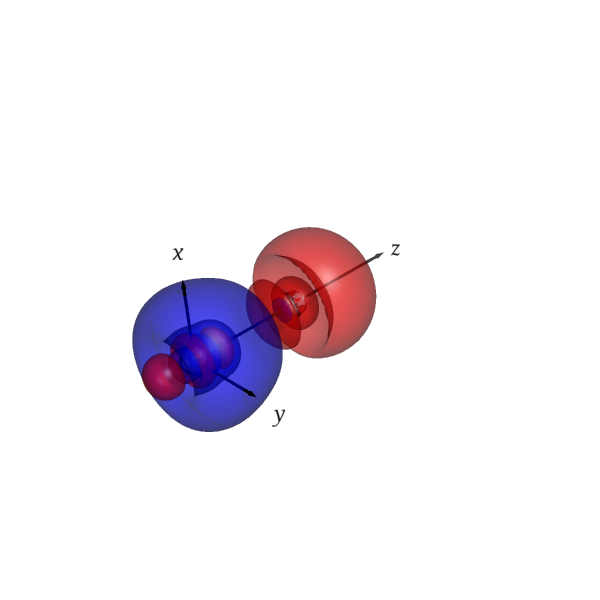
\includegraphics[width=\linewidth]{./AuHg+/pair1.png} 
        \caption*{\ \ \ \ \ \ \ \ $\Delta \rho'_1$} 
    \end{subfigure}

    \vspace{0.0cm}
    \begin{subfigure}[t]{0.30\textwidth}
        \centering
        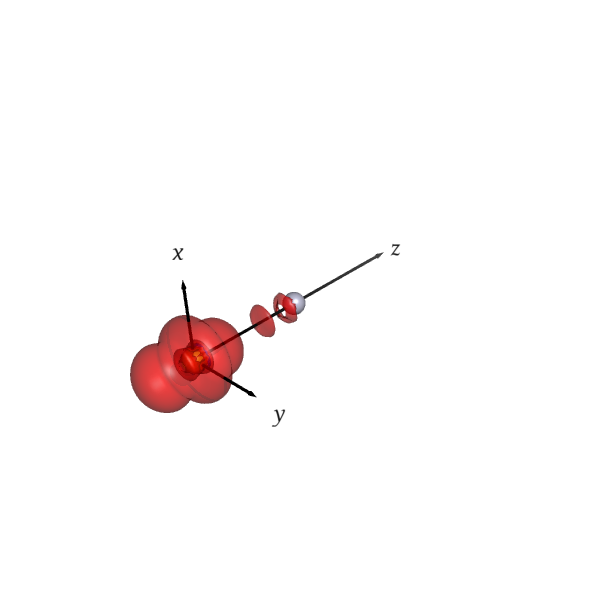
\includegraphics[width=\linewidth]{./AuHg+/nocv-3.png}
        \caption*{\ \ \ \ \ \ \ \ $|\varphi_{-2}|^2$}
    \end{subfigure}
    \hfill
    \begin{subfigure}[t]{0.30\textwidth}
        \centering
        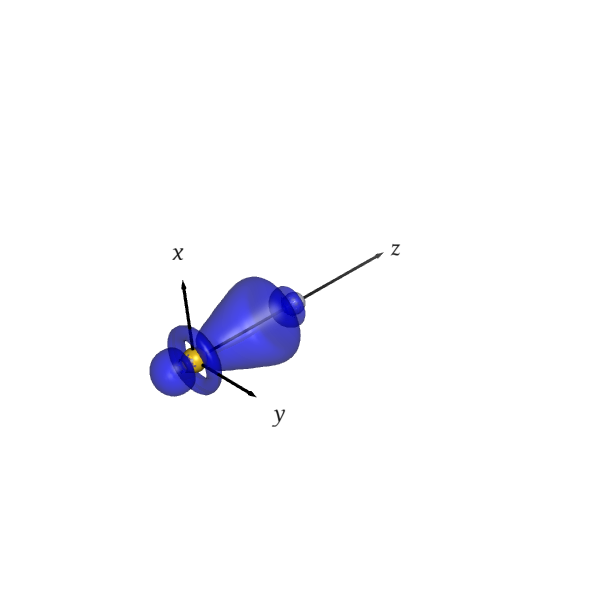
\includegraphics[width=\linewidth]{./AuHg+/nocv+3.png}
        \caption*{\ \ \ \ \ \ \ \ $|\varphi_{+2}|^2$}
    \end{subfigure}
    \hfill
    \begin{subfigure}[t]{0.30\textwidth}
        \centering
        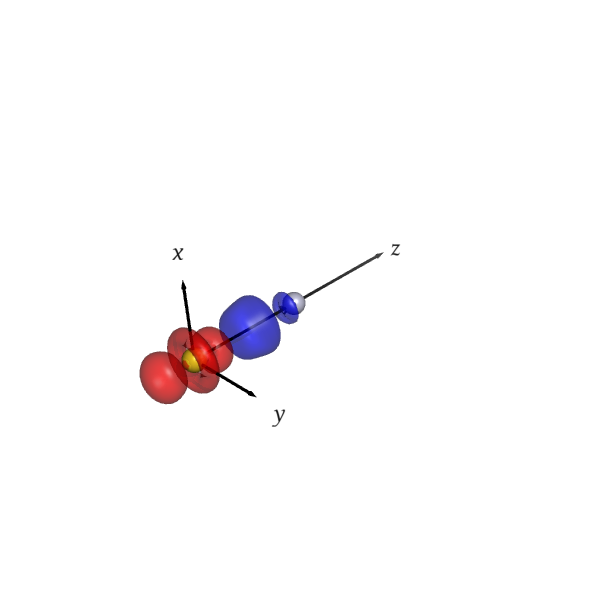
\includegraphics[width=\linewidth]{./AuHg+/pair3.png} 
        \caption*{\ \ \ \ \ \ \ \ $\Delta \rho'_2$} 
    \end{subfigure}

    \vspace{0.0cm}
    \begin{subfigure}[t]{0.30\textwidth}
        \centering
        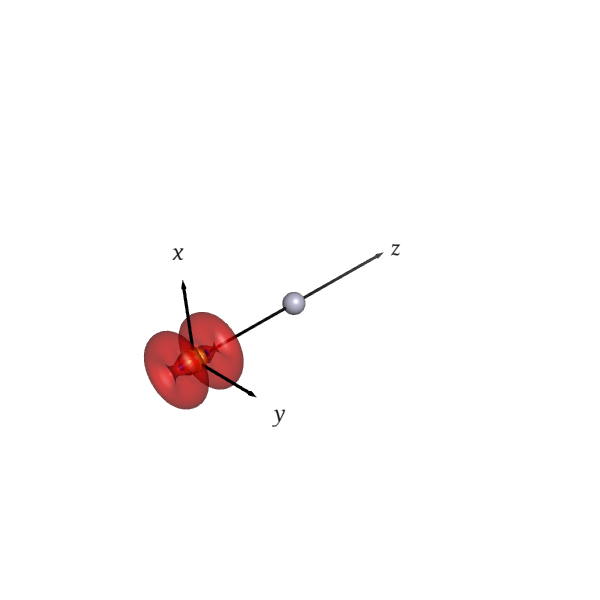
\includegraphics[width=\linewidth]{./AuHg+/nocv-5.png} 
        \caption*{\ \ \ \ \ \ \ \ $|\varphi_{-3}|^2$} 
    \end{subfigure}
    \hfill
    \begin{subfigure}[t]{0.30\textwidth}
        \centering
        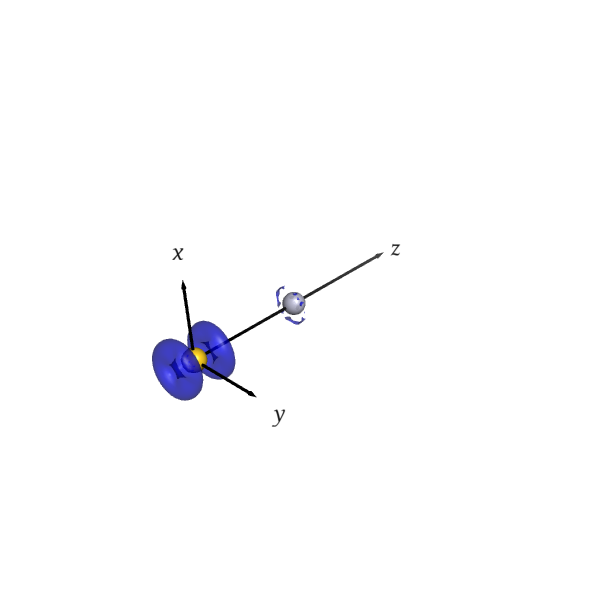
\includegraphics[width=\linewidth]{./AuHg+/nocv+5.png} 
        \caption*{\ \ \ \ \ \ \ \ $|\varphi_{+3}|^2$} 
    \end{subfigure}
    \hfill
    \begin{subfigure}[t]{0.30\textwidth}
        \centering
        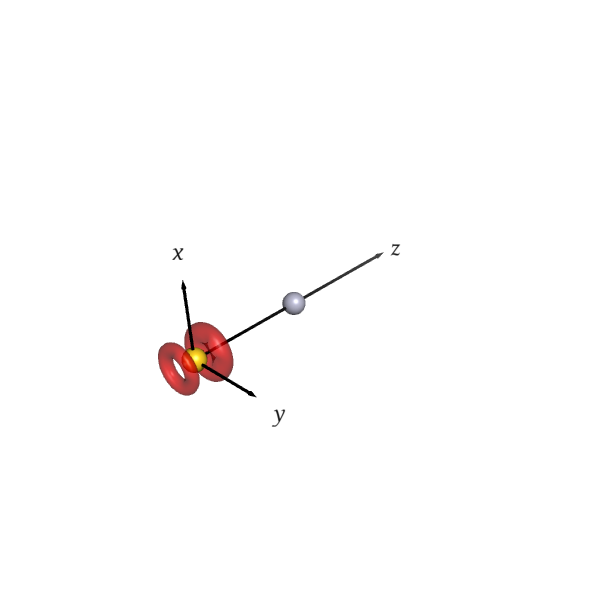
\includegraphics[width=\linewidth]{./AuHg+/pair5.png} 
        \caption*{\ \ \ \ \ \ \ \ $\Delta \rho'_3$} 
    \end{subfigure}

\caption{NOCV pairs for AuHg+ system}
\end{figure}


\begin{figure}[!h]
\includegraphics[angle=-90,width=0.80\textwidth]{./AuCn+/cd.pdf}
\caption{CD curve for AuCn+ system}
\end{figure}
\begin{figure}[!h]
    \centering
    \centering
    \begin{subfigure}[t]{0.33\textwidth}
        \centering
        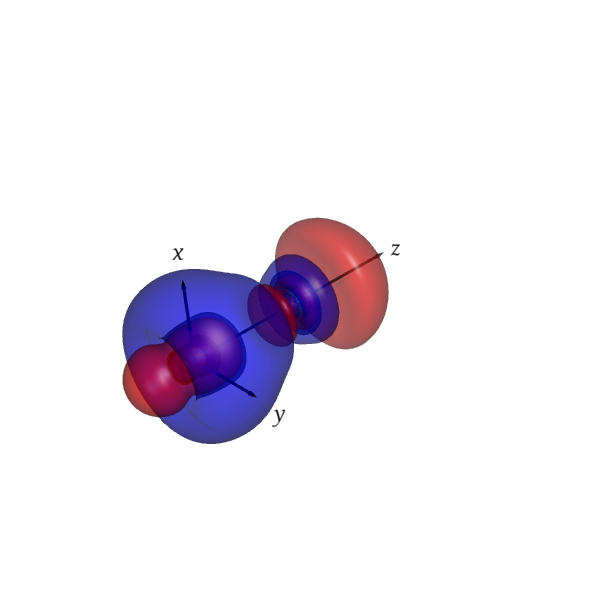
\includegraphics[width=\linewidth]{./AuCn+/diff_tot.png} 
        \caption*{\ \ \ \ \ \ \ \ $\Delta \rho'$} 
    \end{subfigure}
    \hfill
 
    \vspace{0.0cm}
    \begin{subfigure}[t]{0.32\textwidth}
        \centering
        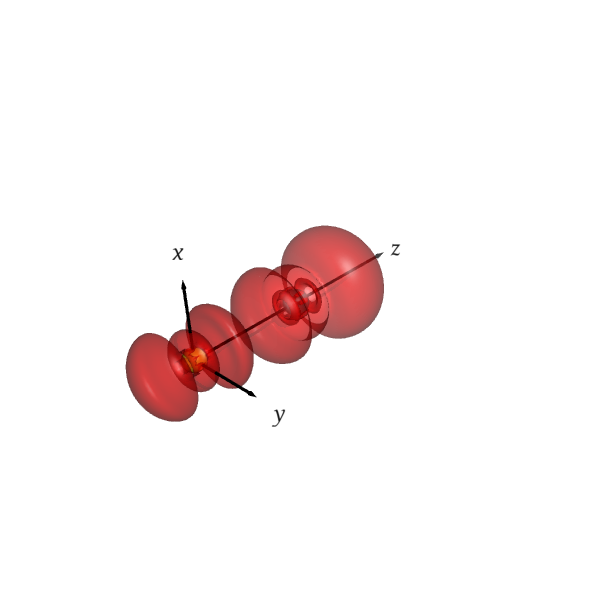
\includegraphics[width=\linewidth]{./AuCn+/nocv-1.png} 
        \caption*{\ \ \ \ \ \ \ \ $|\varphi_{-1}|^2$} 
    \end{subfigure}
    \hfill
    \begin{subfigure}[t]{0.32\textwidth}
        \centering
        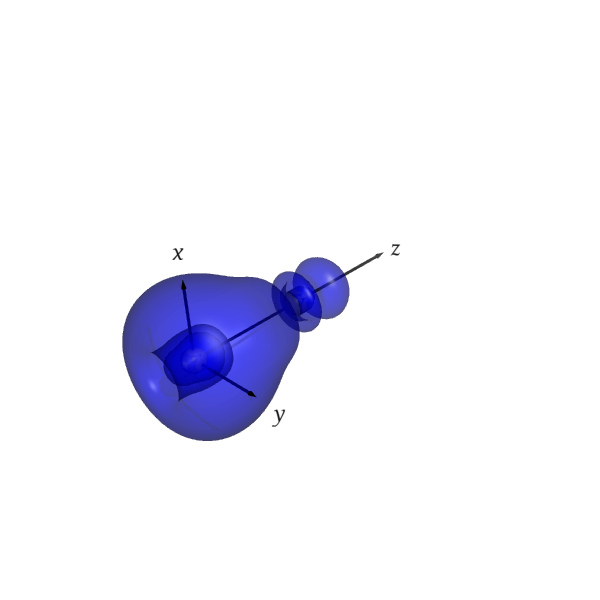
\includegraphics[width=\linewidth]{./AuCn+/nocv+1.png} 
        \caption*{\ \ \ \ \ \ \ \ $|\varphi_{+1}|^2$} 
    \end{subfigure}
    \hfill
    \begin{subfigure}[t]{0.32\textwidth}
        \centering
        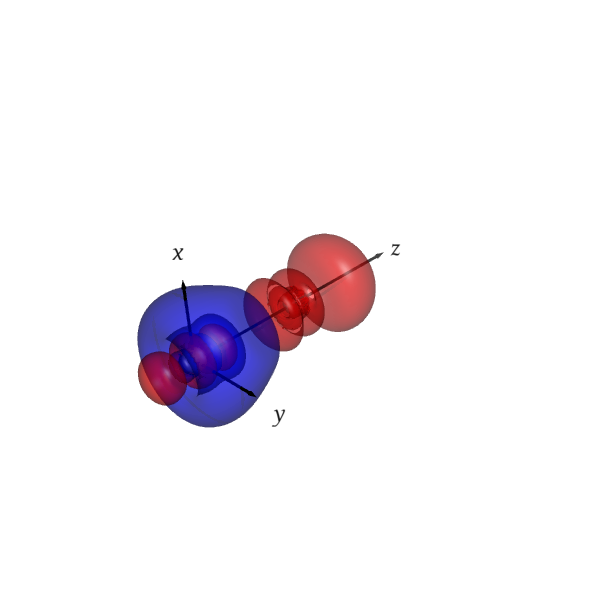
\includegraphics[width=\linewidth]{./AuCn+/pair1.png} 
        \caption*{\ \ \ \ \ \ \ \ $\Delta \rho'_1$} 
    \end{subfigure}

    \vspace{0.0cm}
    \begin{subfigure}[t]{0.32\textwidth}
        \centering
        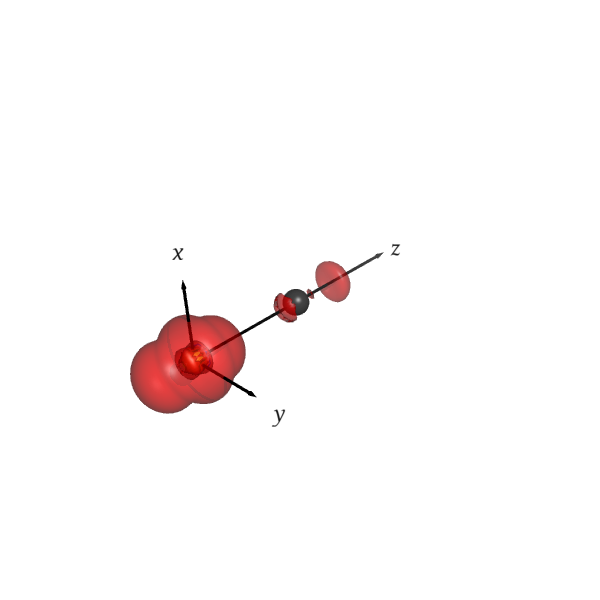
\includegraphics[width=\linewidth]{./AuCn+/nocv-3.png}
        \caption*{\ \ \ \ \ \ \ \ $|\varphi_{-2}|^2$}
    \end{subfigure}
    \hfill
    \begin{subfigure}[t]{0.32\textwidth}
        \centering
        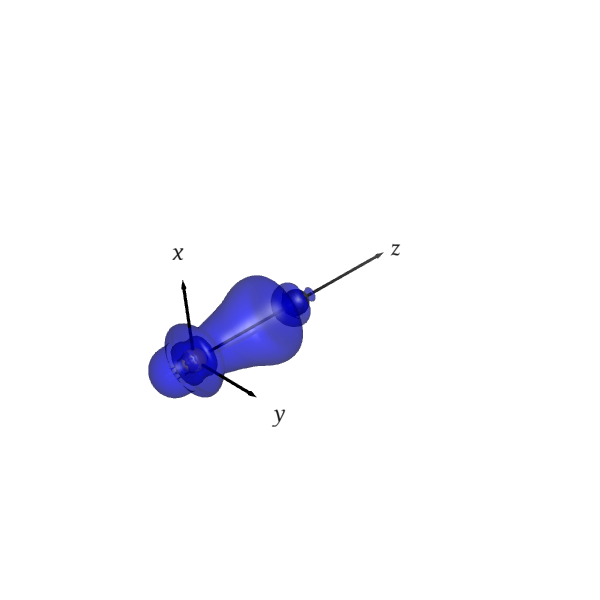
\includegraphics[width=\linewidth]{./AuCn+/nocv+3.png}
        \caption*{\ \ \ \ \ \ \ \ $|\varphi_{+2}|^2$}
    \end{subfigure}
    \hfill
    \begin{subfigure}[t]{0.32\textwidth}
        \centering
        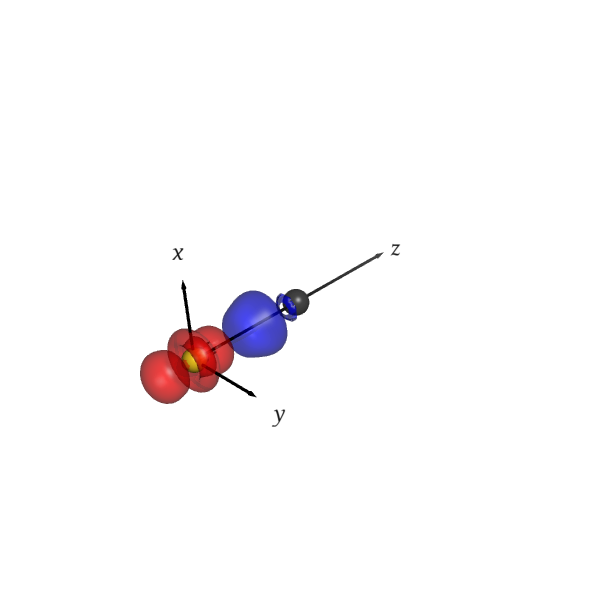
\includegraphics[width=\linewidth]{./AuCn+/pair3.png} 
        \caption*{\ \ \ \ \ \ \ \ $\Delta \rho'_2$} 
    \end{subfigure}

    \vspace{0.0cm}
    \begin{subfigure}[t]{0.32\textwidth}
        \centering
        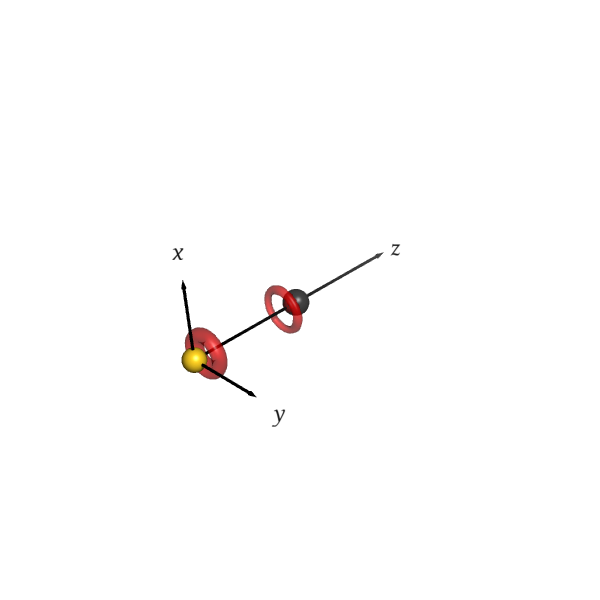
\includegraphics[width=\linewidth]{./AuCn+/nocv-5.png} 
        \caption*{\ \ \ \ \ \ \ \ $|\varphi_{-3}|^2$} 
    \end{subfigure}
    \hfill
    \begin{subfigure}[t]{0.32\textwidth}
        \centering
        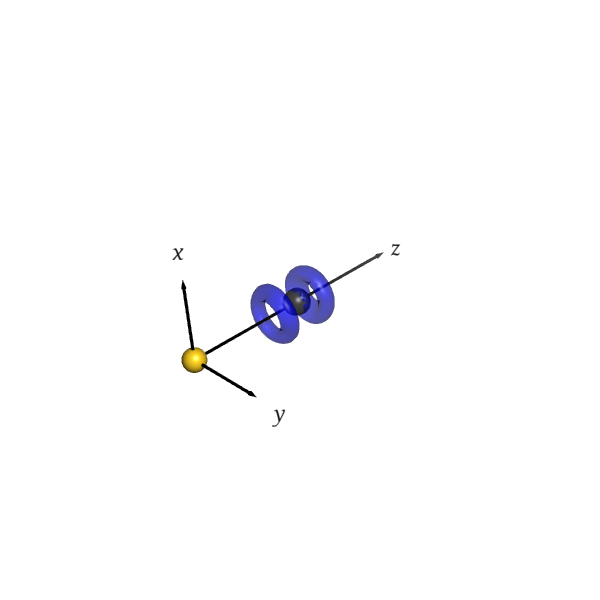
\includegraphics[width=\linewidth]{./AuCn+/nocv+5.png} 
        \caption*{\ \ \ \ \ \ \ \ $|\varphi_{+3}|^2$} 
    \end{subfigure}
    \hfill
    \begin{subfigure}[t]{0.32\textwidth}
        \centering
        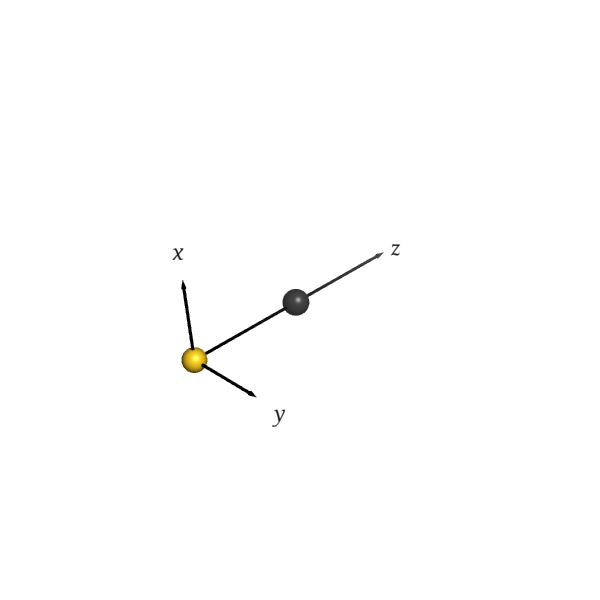
\includegraphics[width=\linewidth]{./AuCn+/pair5.png} 
        \caption*{\ \ \ \ \ \ \ \ $\Delta \rho'_3$} 
    \end{subfigure}

\caption{NOCV pairs for AuCn+ system}
\end{figure}


\begin{figure}[!h]
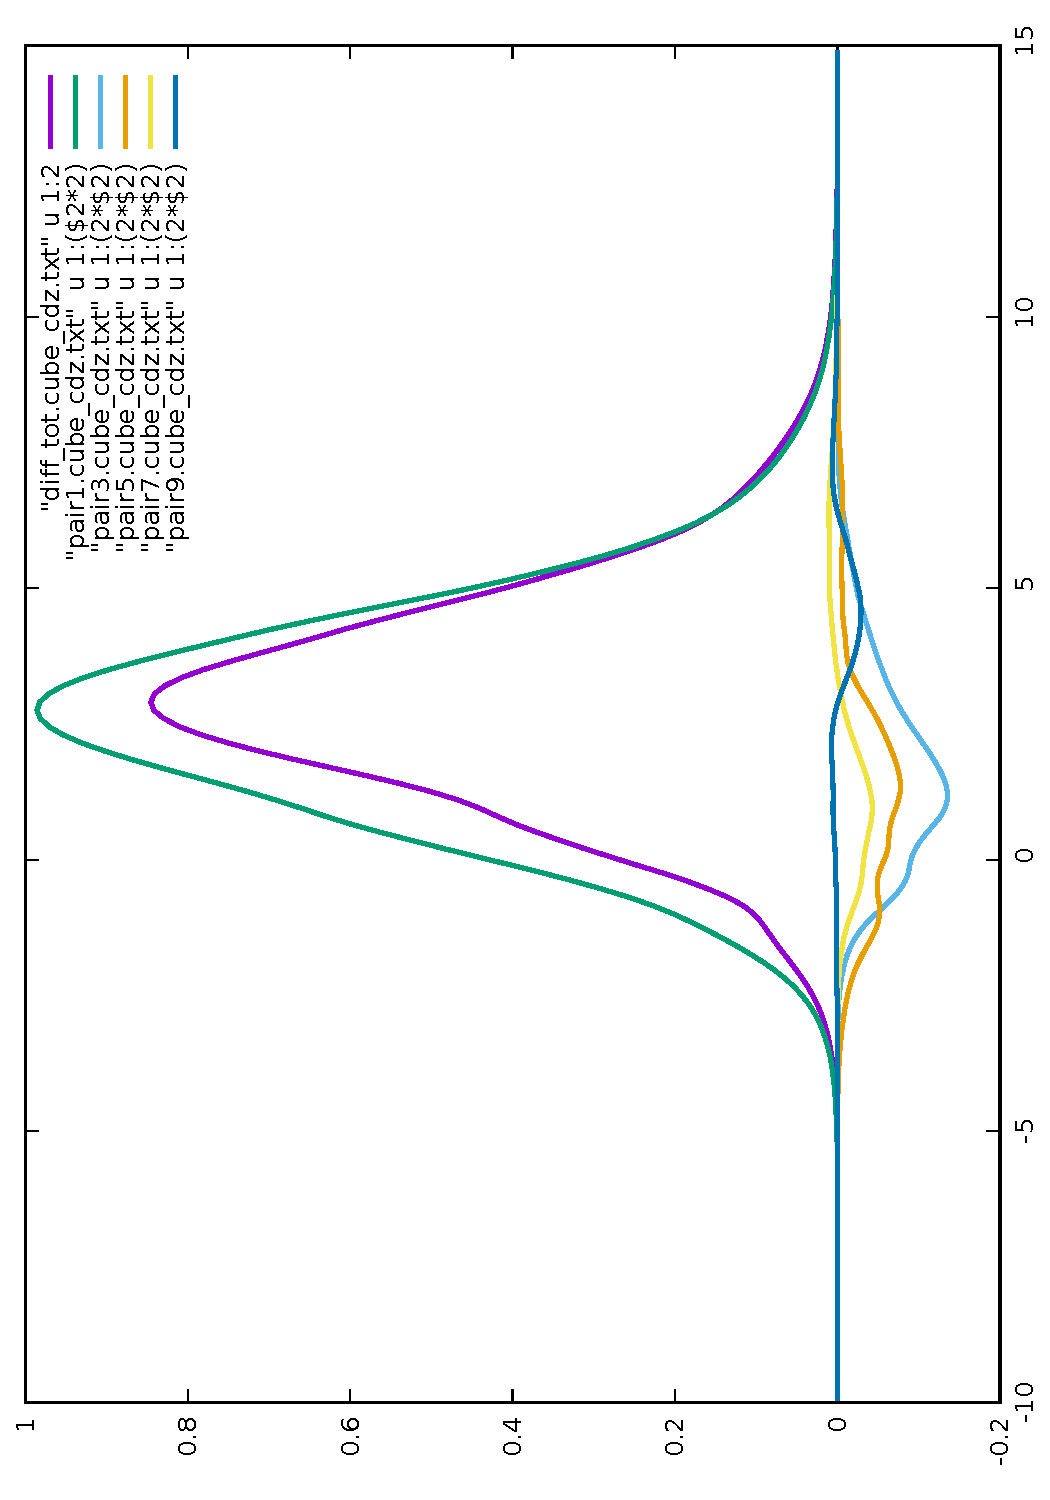
\includegraphics[angle=-90,width=0.80\textwidth]{./AuPb+/cd.pdf}
\caption{CD curve for AuPb+ system}
\end{figure}

\begin{figure}[!h]
    \centering
    \centering
    \begin{subfigure}[t]{0.33\textwidth}
        \centering
        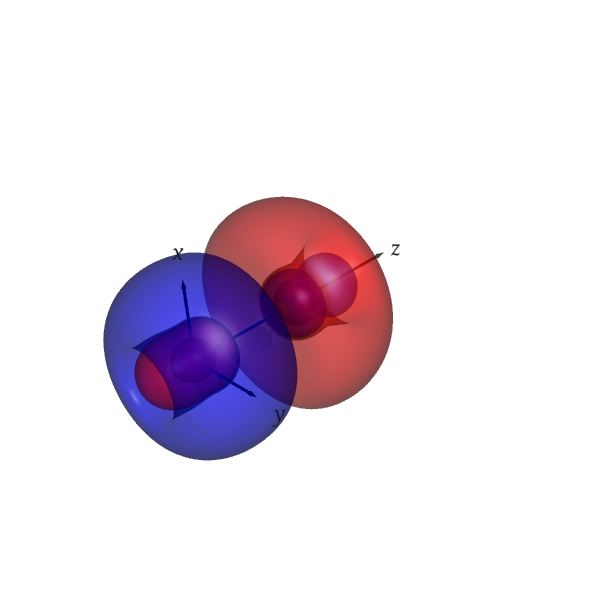
\includegraphics[width=\linewidth]{./AuPb+/diff_tot.png} 
        \caption*{\ \ \ \ \ \ \ \ $\Delta \rho'$} 
    \end{subfigure}
    \hfill
 
    \vspace{0.0cm}
    \begin{subfigure}[t]{0.32\textwidth}
        \centering
        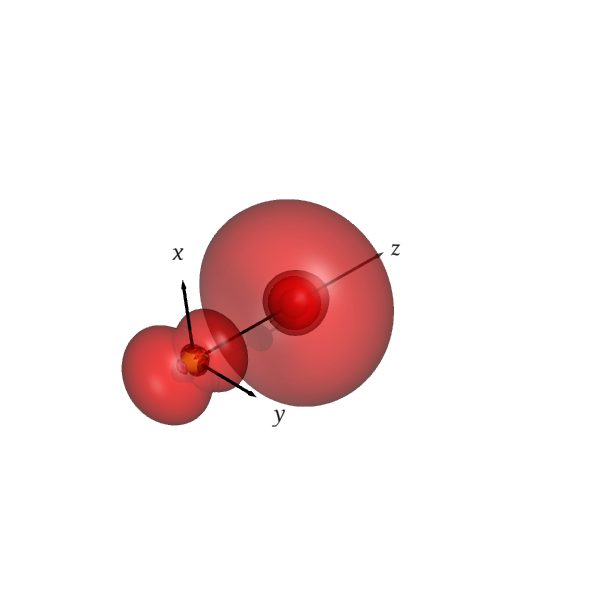
\includegraphics[width=\linewidth]{./AuPb+/nocv-1.png} 
        \caption*{\ \ \ \ \ \ \ \ $|\varphi_{-1}|^2$} 
    \end{subfigure}
    \hfill
    \begin{subfigure}[t]{0.32\textwidth}
        \centering
        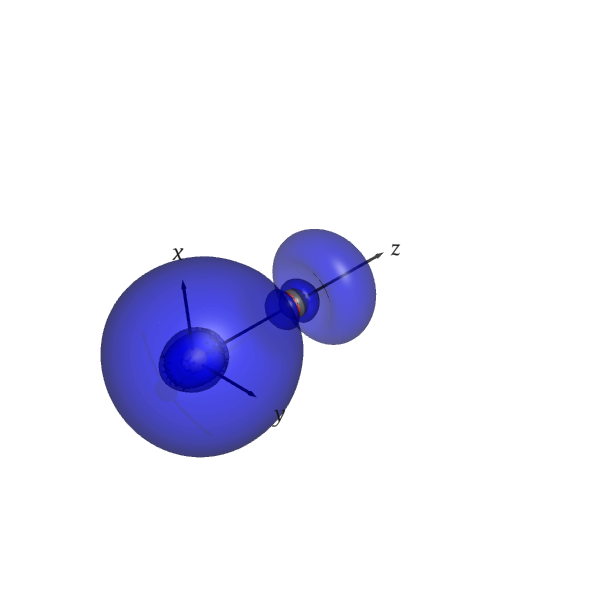
\includegraphics[width=\linewidth]{./AuPb+/nocv+1.png} 
        \caption*{\ \ \ \ \ \ \ \ $|\varphi_{+1}|^2$} 
    \end{subfigure}
    \hfill
    \begin{subfigure}[t]{0.32\textwidth}
        \centering
        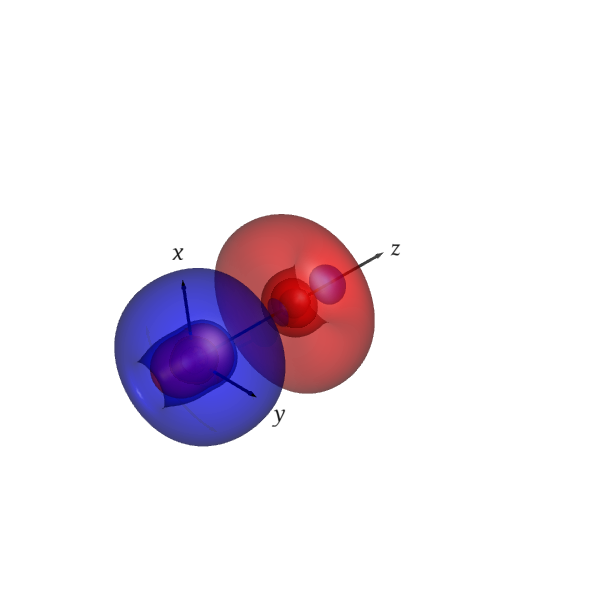
\includegraphics[width=\linewidth]{./AuPb+/pair1.png} 
        \caption*{\ \ \ \ \ \ \ \ $\Delta \rho'_1$} 
    \end{subfigure}

    \vspace{0.0cm}
    \begin{subfigure}[t]{0.32\textwidth}
        \centering
        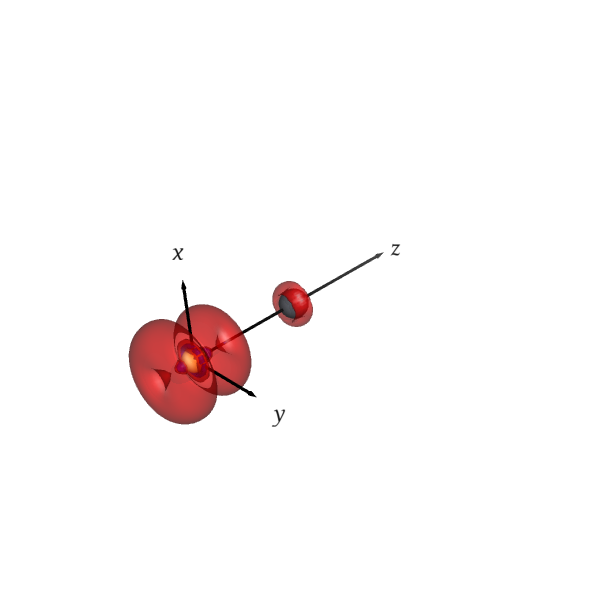
\includegraphics[width=\linewidth]{./AuPb+/nocv-3.png}
        \caption*{\ \ \ \ \ \ \ \ $|\varphi_{-2}|^2$}
    \end{subfigure}
    \hfill
    \begin{subfigure}[t]{0.32\textwidth}
        \centering
        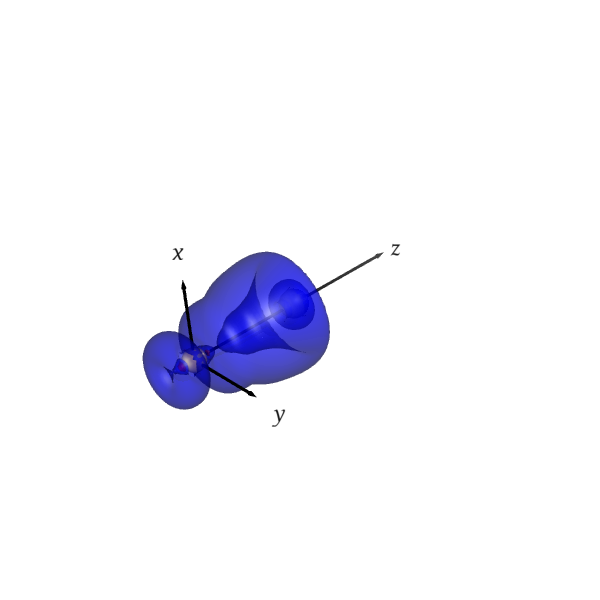
\includegraphics[width=\linewidth]{./AuPb+/nocv+3.png}
        \caption*{\ \ \ \ \ \ \ \ $|\varphi_{+2}|^2$}
    \end{subfigure}
    \hfill
    \begin{subfigure}[t]{0.32\textwidth}
        \centering
        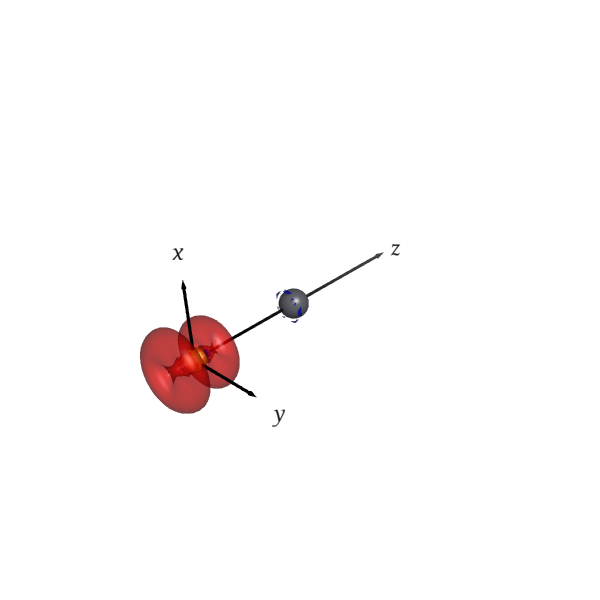
\includegraphics[width=\linewidth]{./AuPb+/pair3.png} 
        \caption*{\ \ \ \ \ \ \ \ $\Delta \rho'_2$} 
    \end{subfigure}

    \vspace{0.0cm}
    \begin{subfigure}[t]{0.32\textwidth}
        \centering
        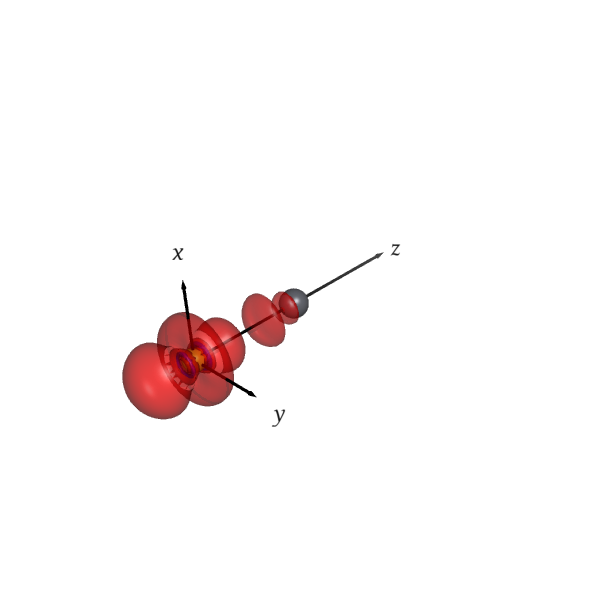
\includegraphics[width=\linewidth]{./AuPb+/nocv-5.png} 
        \caption*{\ \ \ \ \ \ \ \ $|\varphi_{-3}|^2$} 
    \end{subfigure}
    \hfill
    \begin{subfigure}[t]{0.32\textwidth}
        \centering
        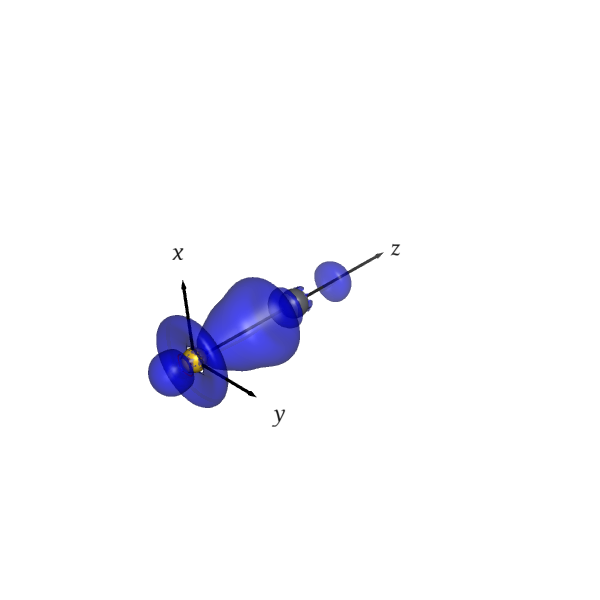
\includegraphics[width=\linewidth]{./AuPb+/nocv+5.png} 
        \caption*{\ \ \ \ \ \ \ \ $|\varphi_{+3}|^2$} 
    \end{subfigure}
    \hfill
    \begin{subfigure}[t]{0.32\textwidth}
        \centering
        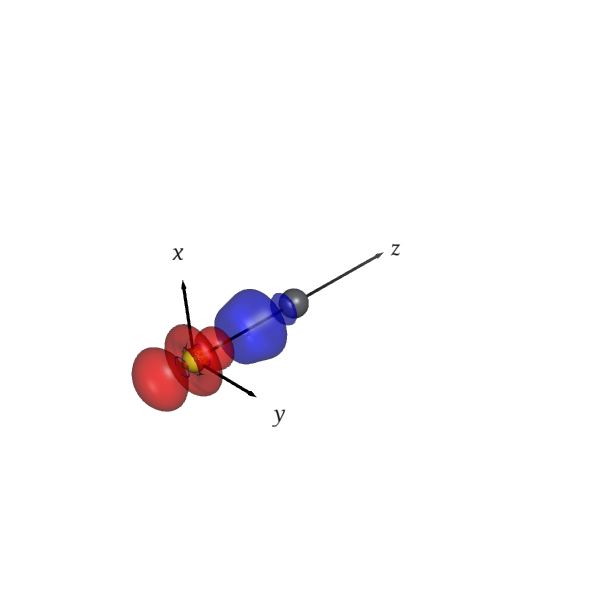
\includegraphics[width=\linewidth]{./AuPb+/pair5.png} 
        \caption*{\ \ \ \ \ \ \ \ $\Delta \rho'_3$} 
    \end{subfigure}

\caption{NOCV pairs for AuPb+ system}
\end{figure}


\begin{figure}[!h]
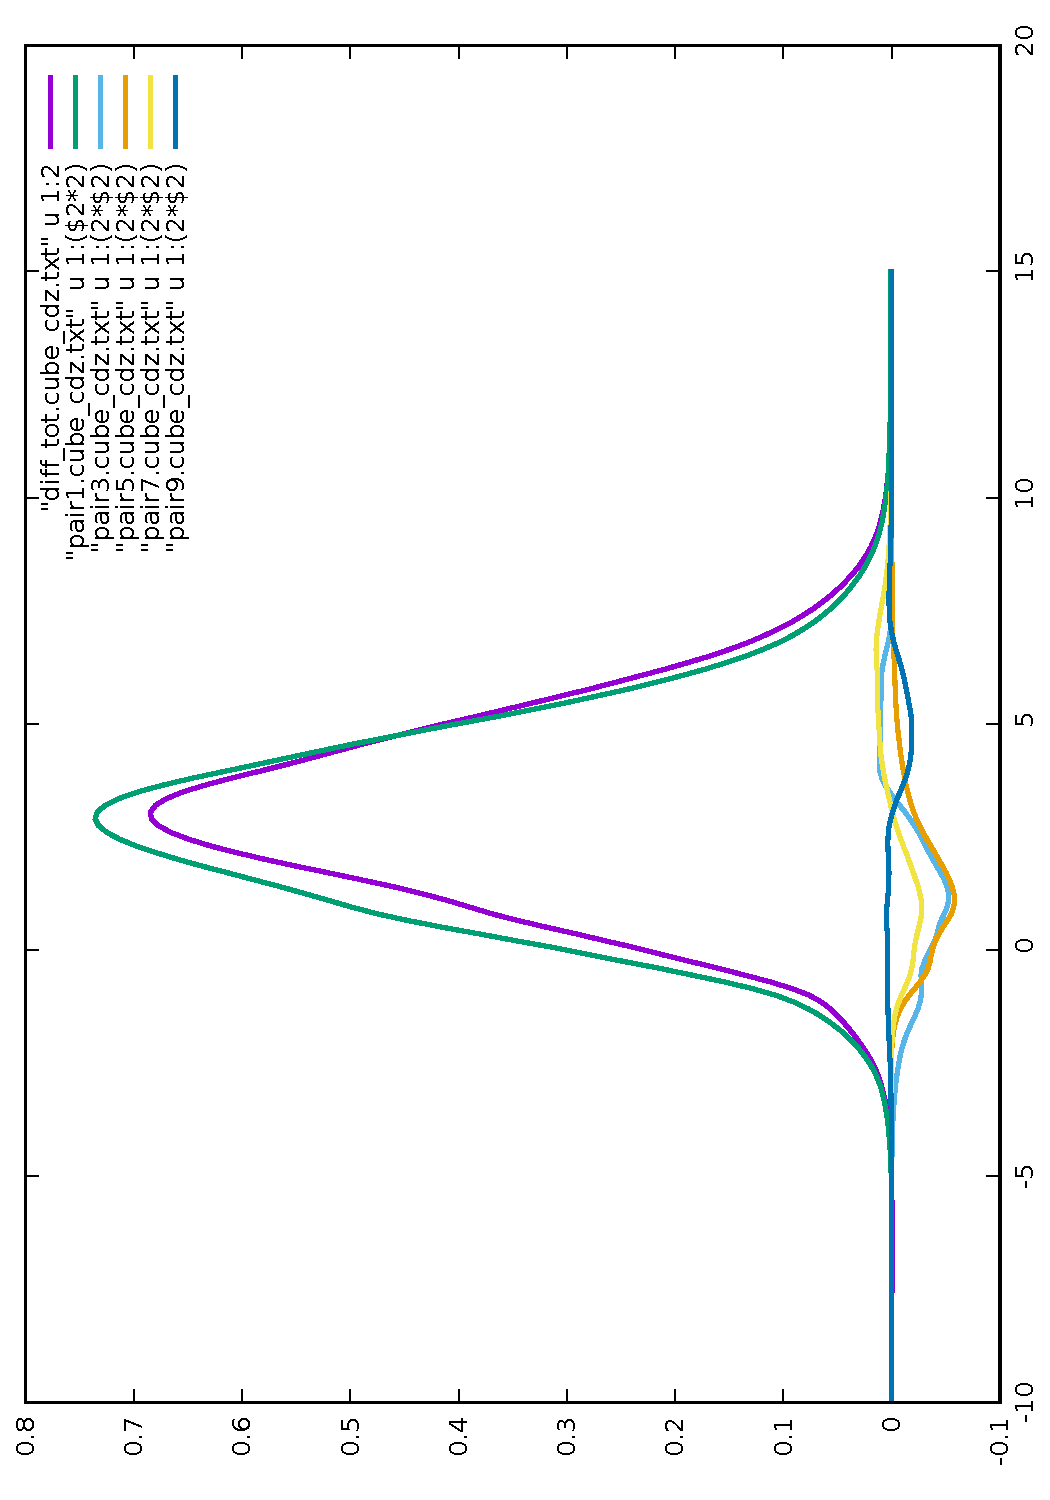
\includegraphics[angle=-90,width=0.80\textwidth]{./AuFl+/cd.pdf}
\caption{CD curve for AuFl+ system}
\end{figure}

\begin{figure}[!h]
    \centering
    \centering
    \begin{subfigure}[t]{0.33\textwidth}
        \centering
        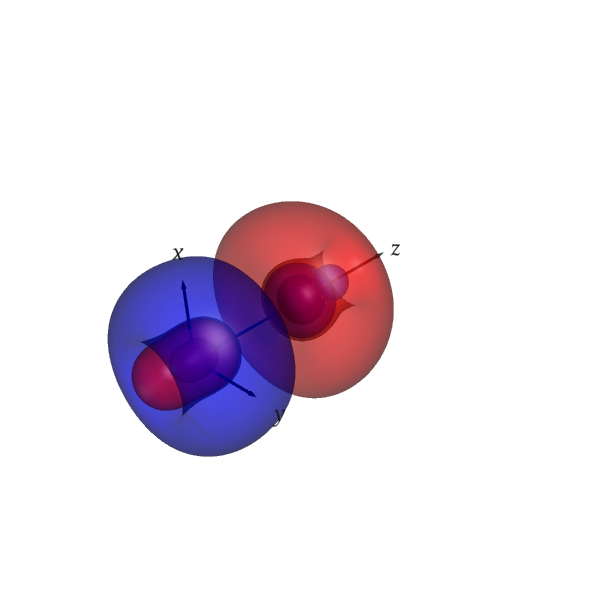
\includegraphics[width=\linewidth]{./AuFl+/diff_tot.png} 
        \caption*{\ \ \ \ \ \ \ \ $\Delta \rho'$} 
    \end{subfigure}
    \hfill
 
    \vspace{0.0cm}
    \begin{subfigure}[t]{0.32\textwidth}
        \centering
        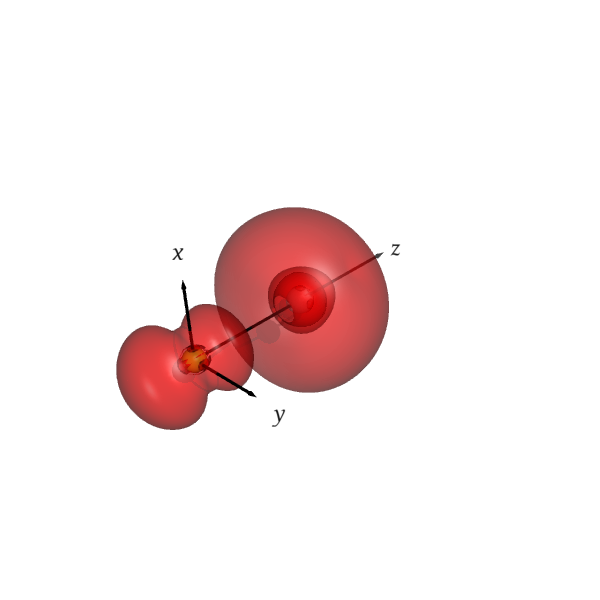
\includegraphics[width=\linewidth]{./AuFl+/nocv-1.png} 
        \caption*{\ \ \ \ \ \ \ \ $|\varphi_{-1}|^2$} 
    \end{subfigure}
    \hfill
    \begin{subfigure}[t]{0.32\textwidth}
        \centering
        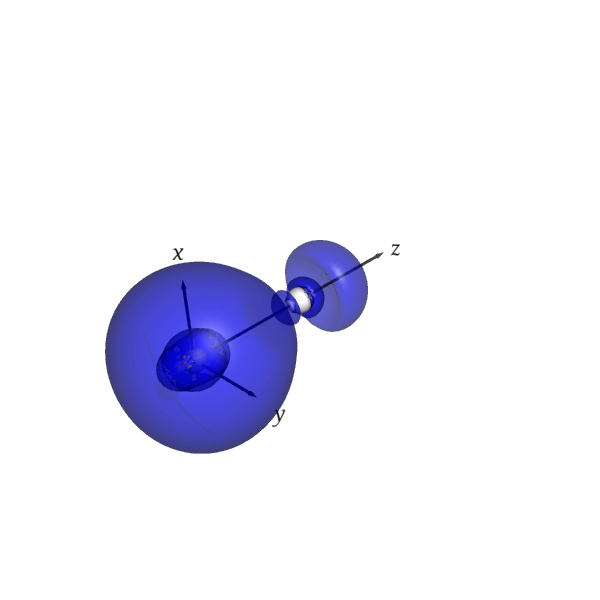
\includegraphics[width=\linewidth]{./AuFl+/nocv+1.png} 
        \caption*{\ \ \ \ \ \ \ \ $|\varphi_{+1}|^2$} 
    \end{subfigure}
    \hfill
    \begin{subfigure}[t]{0.32\textwidth}
        \centering
        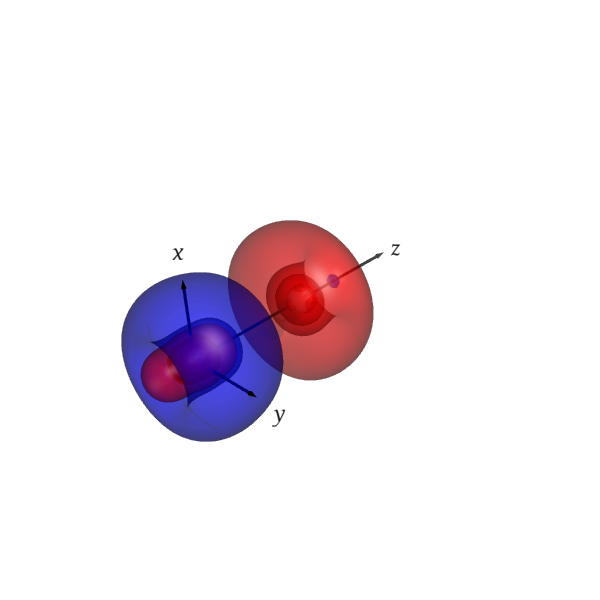
\includegraphics[width=\linewidth]{./AuFl+/pair1.png} 
        \caption*{\ \ \ \ \ \ \ \ $\Delta \rho'_1$} 
    \end{subfigure}

    \vspace{0.0cm}
    \begin{subfigure}[t]{0.32\textwidth}
        \centering
        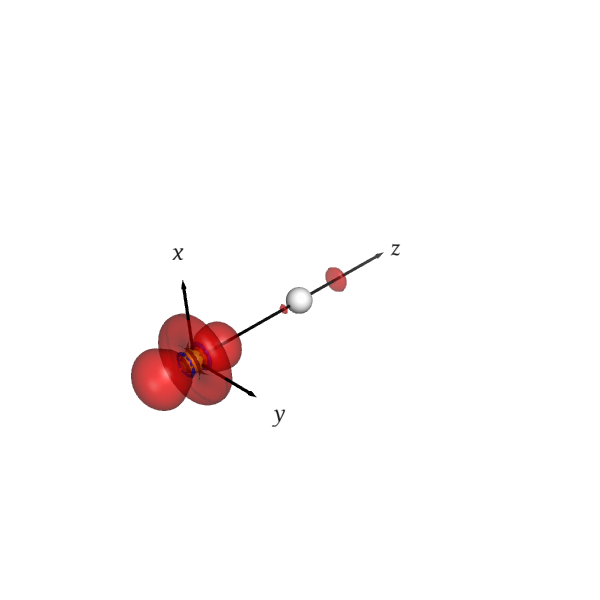
\includegraphics[width=\linewidth]{./AuFl+/nocv-3.png}
        \caption*{\ \ \ \ \ \ \ \ $|\varphi_{-2}|^2$}
    \end{subfigure}
    \hfill
    \begin{subfigure}[t]{0.32\textwidth}
        \centering
        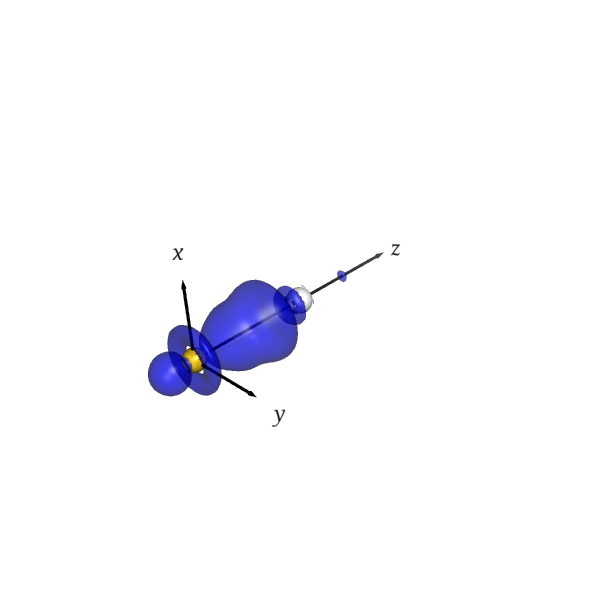
\includegraphics[width=\linewidth]{./AuFl+/nocv+3.png}
        \caption*{\ \ \ \ \ \ \ \ $|\varphi_{+2}|^2$}
    \end{subfigure}
    \hfill
    \begin{subfigure}[t]{0.32\textwidth}
        \centering
        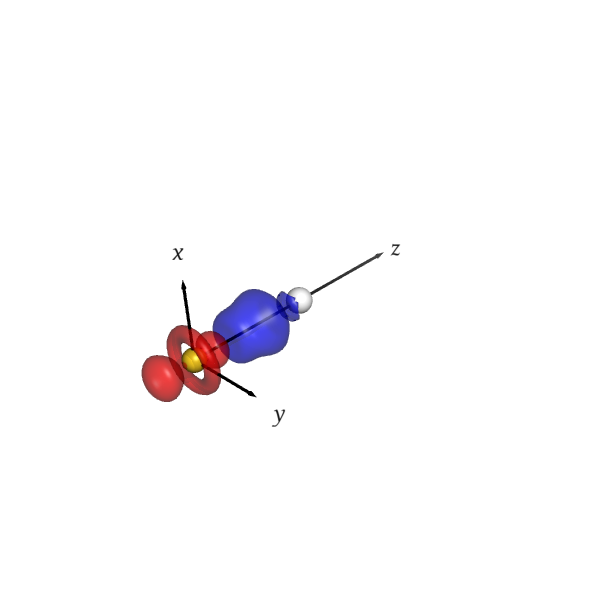
\includegraphics[width=\linewidth]{./AuFl+/pair3.png} 
        \caption*{\ \ \ \ \ \ \ \ $\Delta \rho'_2$} 
    \end{subfigure}

    \vspace{0.0cm}
    \begin{subfigure}[t]{0.32\textwidth}
        \centering
        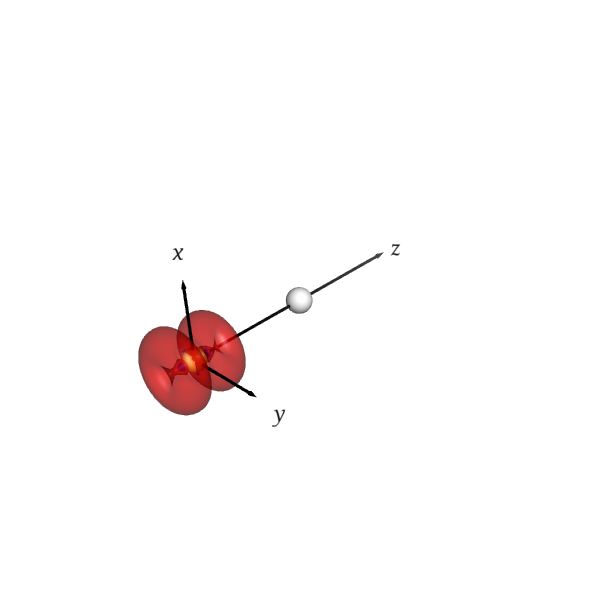
\includegraphics[width=\linewidth]{./AuFl+/nocv-5.png} 
        \caption*{\ \ \ \ \ \ \ \ $|\varphi_{-3}|^2$} 
    \end{subfigure}
    \hfill
    \begin{subfigure}[t]{0.32\textwidth}
        \centering
        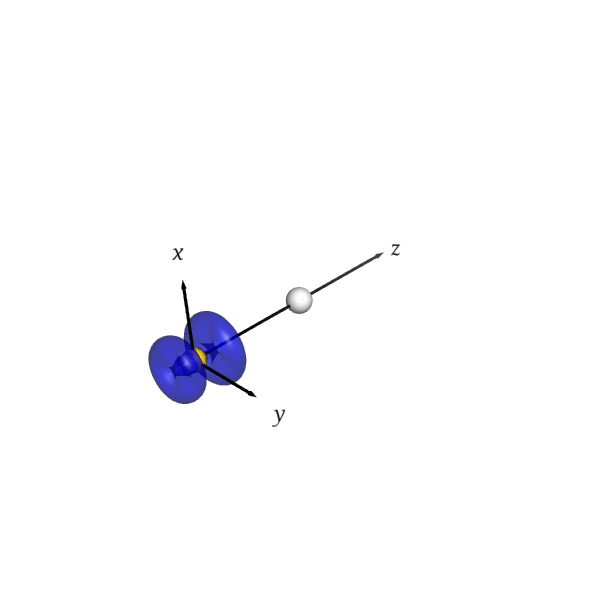
\includegraphics[width=\linewidth]{./AuFl+/nocv+5.png} 
        \caption*{\ \ \ \ \ \ \ \ $|\varphi_{+3}|^2$} 
    \end{subfigure}
    \hfill
    \begin{subfigure}[t]{0.32\textwidth}
        \centering
        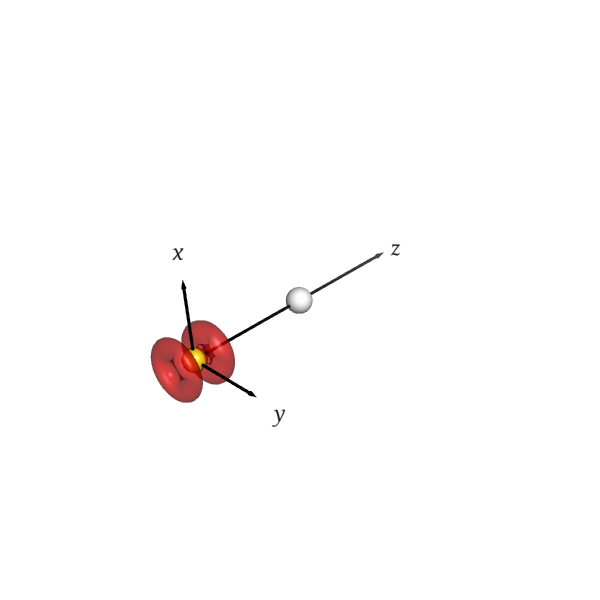
\includegraphics[width=\linewidth]{./AuFl+/pair5.png} 
        \caption*{\ \ \ \ \ \ \ \ $\Delta \rho'_3$} 
    \end{subfigure}

\caption{NOCV pairs for AuFl+ system}
\end{figure}


\begin{figure}[!h]
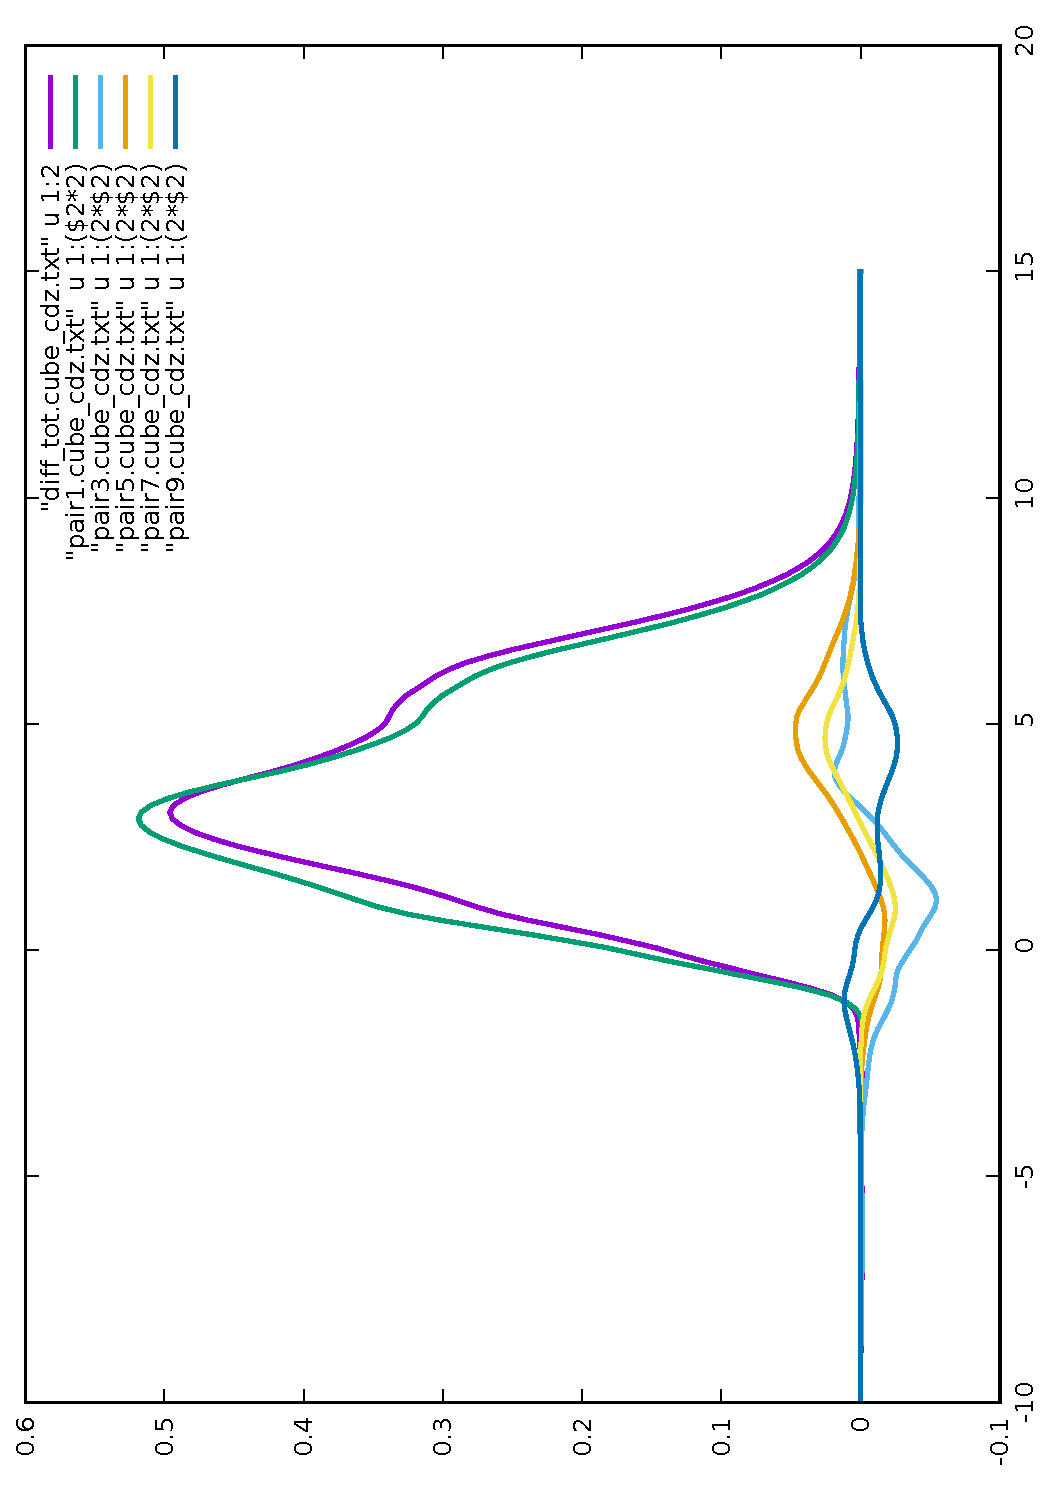
\includegraphics[angle=-90,width=0.80\textwidth]{./AuRn+/cd.pdf}
\caption{CD curve for AuRn+ system}
\end{figure}

\begin{figure}[!h]
    \centering
    \centering
    \begin{subfigure}[t]{0.33\textwidth}
        \centering
        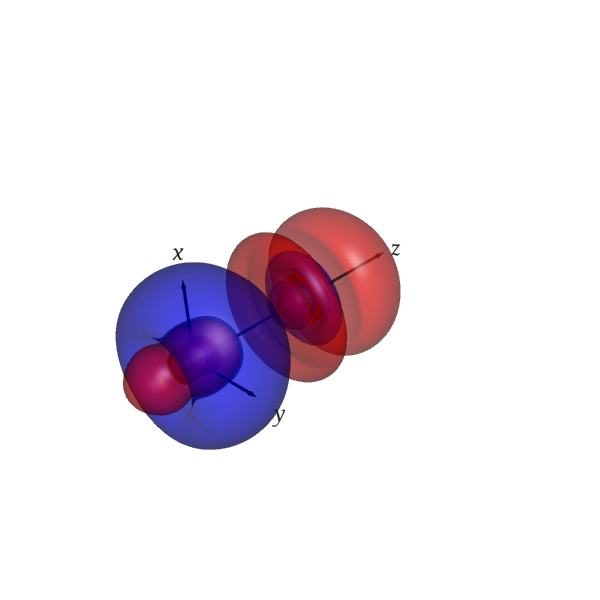
\includegraphics[width=\linewidth]{./AuRn+/diff_tot.png} 
        \caption*{\ \ \ \ \ \ \ \ $\Delta \rho'$} 
    \end{subfigure}
    \hfill
 
    \vspace{0.0cm}
    \begin{subfigure}[t]{0.32\textwidth}
        \centering
        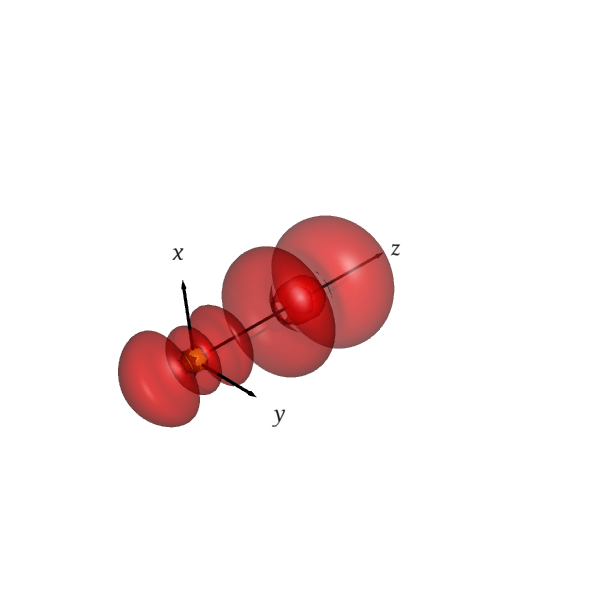
\includegraphics[width=\linewidth]{./AuRn+/nocv-1.png} 
        \caption*{\ \ \ \ \ \ \ \ $|\varphi_{-1}|^2$} 
    \end{subfigure}
    \hfill
    \begin{subfigure}[t]{0.32\textwidth}
        \centering
        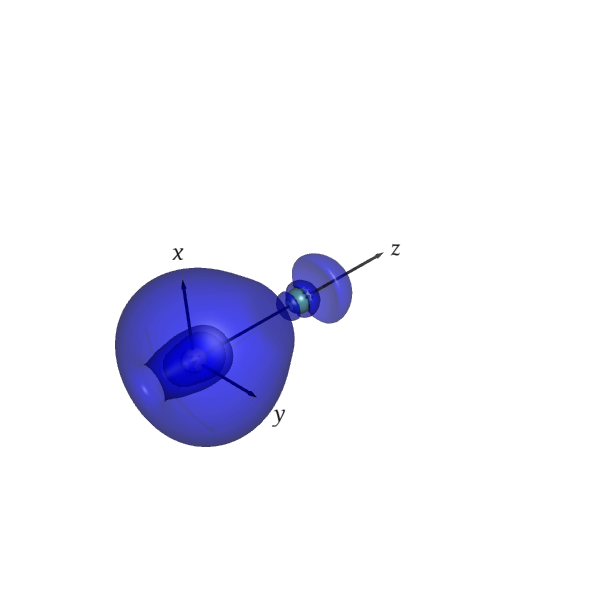
\includegraphics[width=\linewidth]{./AuRn+/nocv+1.png} 
        \caption*{\ \ \ \ \ \ \ \ $|\varphi_{+1}|^2$} 
    \end{subfigure}
    \hfill
    \begin{subfigure}[t]{0.32\textwidth}
        \centering
        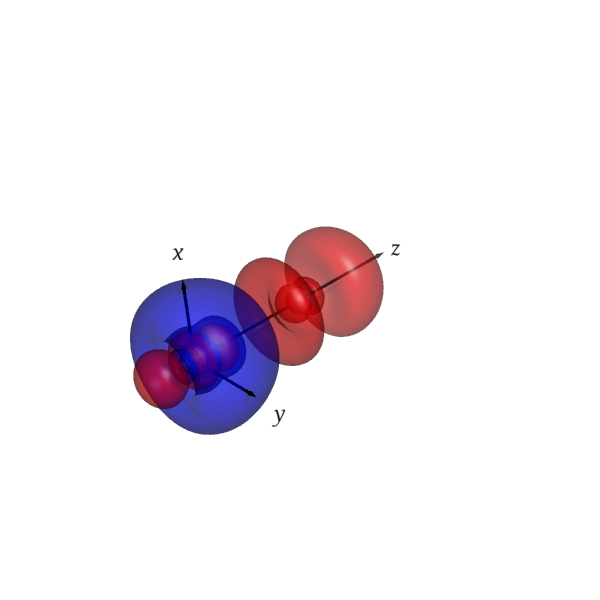
\includegraphics[width=\linewidth]{./AuRn+/pair1.png} 
        \caption*{\ \ \ \ \ \ \ \ $\Delta \rho'_1$} 
    \end{subfigure}

    \vspace{0.0cm}
    \begin{subfigure}[t]{0.32\textwidth}
        \centering
        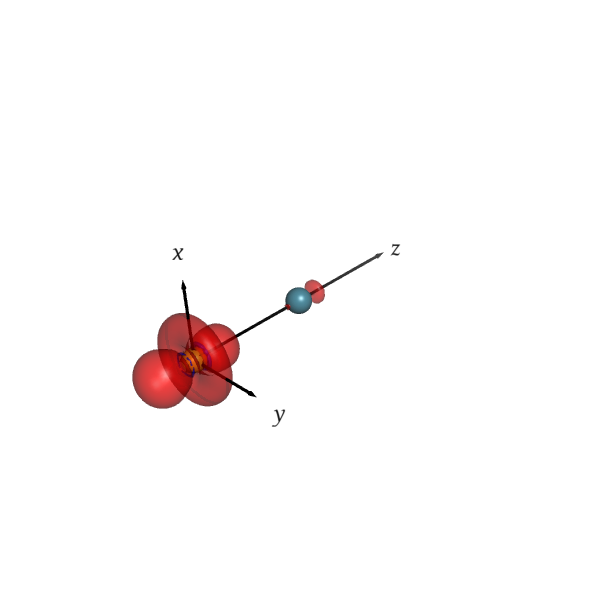
\includegraphics[width=\linewidth]{./AuRn+/nocv-3.png}
        \caption*{\ \ \ \ \ \ \ \ $|\varphi_{-2}|^2$}
    \end{subfigure}
    \hfill
    \begin{subfigure}[t]{0.32\textwidth}
        \centering
        \includegraphics[width=\linewidth]{./AuRn+/nocv+3.png}
        \caption*{\ \ \ \ \ \ \ \ $|\varphi_{+2}|^2$}
    \end{subfigure}
    \hfill
    \begin{subfigure}[t]{0.32\textwidth}
        \centering
        \includegraphics[width=\linewidth]{./AuRn+/pair3.png} 
        \caption*{\ \ \ \ \ \ \ \ $\Delta \rho'_2$} 
    \end{subfigure}

    \vspace{0.0cm}
    \begin{subfigure}[t]{0.32\textwidth}
        \centering
        \includegraphics[width=\linewidth]{./AuRn+/nocv-5.png} 
        \caption*{\ \ \ \ \ \ \ \ $|\varphi_{-3}|^2$} 
    \end{subfigure}
    \hfill
    \begin{subfigure}[t]{0.32\textwidth}
        \centering
        \includegraphics[width=\linewidth]{./AuRn+/nocv+5.png} 
        \caption*{\ \ \ \ \ \ \ \ $|\varphi_{+3}|^2$} 
    \end{subfigure}
    \hfill
    \begin{subfigure}[t]{0.32\textwidth}
        \centering
        \includegraphics[width=\linewidth]{./AuRn+/pair5.png} 
        \caption*{\ \ \ \ \ \ \ \ $\Delta \rho'_3$} 
    \end{subfigure}

\caption{NOCV pairs for AuRn+ system}
\end{figure}


\begin{figure}[!h]
\includegraphics[angle=-90,width=0.80\textwidth]{./AuOg+/cd.pdf}
\caption{CD curve for AuOg+ system}
\end{figure}

\begin{figure}[!h]
    \centering
    \centering
    \begin{subfigure}[t]{0.33\textwidth}
        \centering
        \includegraphics[width=\linewidth]{./AuOg+/diff_tot.png} 
        \caption*{\ \ \ \ \ \ \ \ $\Delta \rho'$} 
    \end{subfigure}
    \hfill
 
    \vspace{0.0cm}
    \begin{subfigure}[t]{0.32\textwidth}
        \centering
        \includegraphics[width=\linewidth]{./AuOg+/nocv-1.png} 
        \caption*{\ \ \ \ \ \ \ \ $|\varphi_{-1}|^2$} 
    \end{subfigure}
    \hfill
    \begin{subfigure}[t]{0.32\textwidth}
        \centering
        \includegraphics[width=\linewidth]{./AuOg+/nocv+1.png} 
        \caption*{\ \ \ \ \ \ \ \ $|\varphi_{+1}|^2$} 
    \end{subfigure}
    \hfill
    \begin{subfigure}[t]{0.32\textwidth}
        \centering
        \includegraphics[width=\linewidth]{./AuOg+/pair1.png} 
        \caption*{\ \ \ \ \ \ \ \ $\Delta \rho'_1$} 
    \end{subfigure}

    \vspace{0.0cm}
    \begin{subfigure}[t]{0.32\textwidth}
        \centering
        \includegraphics[width=\linewidth]{./AuOg+/nocv-3.png}
        \caption*{\ \ \ \ \ \ \ \ $|\varphi_{-2}|^2$}
    \end{subfigure}
    \hfill
    \begin{subfigure}[t]{0.32\textwidth}
        \centering
        \includegraphics[width=\linewidth]{./AuOg+/nocv+3.png}
        \caption*{\ \ \ \ \ \ \ \ $|\varphi_{+2}|^2$}
    \end{subfigure}
    \hfill
    \begin{subfigure}[t]{0.32\textwidth}
        \centering
        \includegraphics[width=\linewidth]{./AuOg+/pair3.png} 
        \caption*{\ \ \ \ \ \ \ \ $\Delta \rho'_2$} 
    \end{subfigure}

    \vspace{0.0cm}
    \begin{subfigure}[t]{0.32\textwidth}
        \centering
        \includegraphics[width=\linewidth]{./AuOg+/nocv-5.png} 
        \caption*{\ \ \ \ \ \ \ \ $|\varphi_{-3}|^2$} 
    \end{subfigure}
    \hfill
    \begin{subfigure}[t]{0.32\textwidth}
        \centering
        \includegraphics[width=\linewidth]{./AuOg+/nocv+5.png} 
        \caption*{\ \ \ \ \ \ \ \ $|\varphi_{+3}|^2$} 
    \end{subfigure}
    \hfill
    \begin{subfigure}[t]{0.32\textwidth}
        \centering
        \includegraphics[width=\linewidth]{./AuOg+/pair5.png} 
        \caption*{\ \ \ \ \ \ \ \ $\Delta \rho'_3$} 
    \end{subfigure}

\caption{NOCV pairs for AuOg+ system}
\end{figure}


\section{A case study the ClAuX (X=Hg, Pb, Rn, Cn, Fl, Og) systems  }


The same approch as before has been used for basis and auxiliary fitting sets.


\section{Conclusions}

\end{document}
